
\begin{frame}
	\frametitle{SNN and the Planar snake car model}
	\begin{itemize}
		\item Spiking Neuronal Networks are promising for robotics
		\item \textbf{BUT} they can't be trained using gradient descend methods
		\item Snake-like robots are very mobile
		\item Simple planar snake robot with slithering gait model and wheels
		\item Highlevel controll using SNN
	\end{itemize}
\end{frame}

\begin{frame}
	\frametitle{Task: Target Tracking}
	\begin{columns}
		\column{0.5\linewidth}
			\begin{itemize}
				\item <1-> Target Tracking
				\item <2-> Prevent collisions with walls
			\end{itemize}
		\column{0.5\linewidth}
			\begin{overprint}
				\onslide<1>
				\begin{figure}
					\centering
					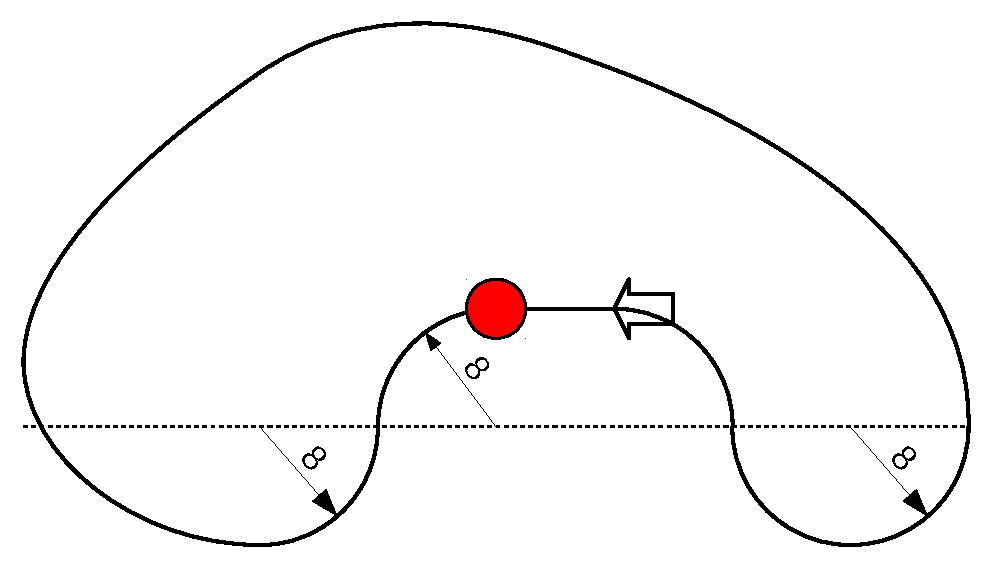
\includegraphics[width=\textwidth]{img/eval_path_tf.pdf}
					\caption{Target tracking SNN evaluation environment.}
					\label{fig:eval_path_tf}
				\end{figure}
				\onslide<2>
				\begin{figure}
					\centering
					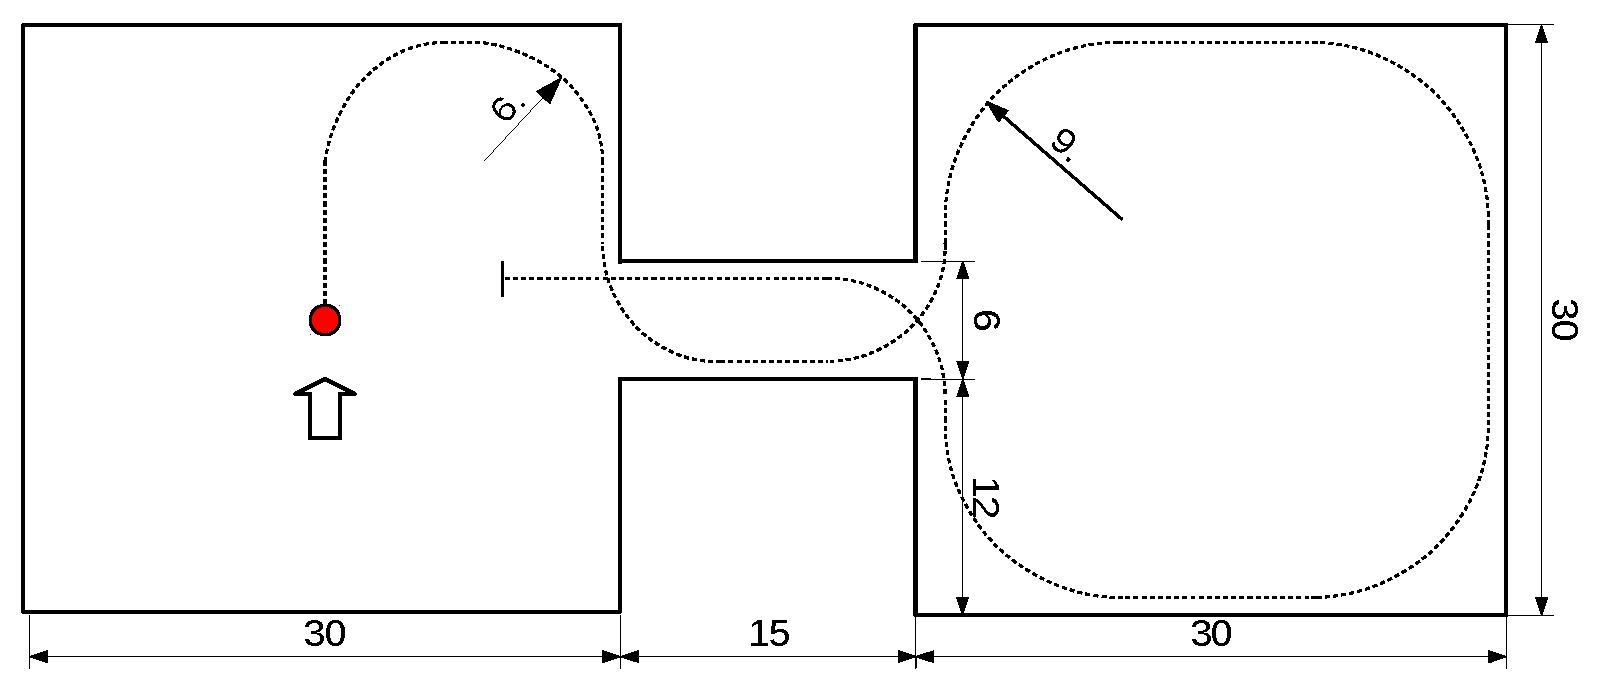
\includegraphics[width=\textwidth]{img/eval_path.pdf}
					\caption{Evaluation environment}
					\label{fig:eval_path}
				\end{figure}
			\end{overprint}
	\end{columns}
\end{frame}

\begin{frame}
	\frametitle{Target Following SNN}
	\begin{columns}
		\column{0.5\linewidth}
			\begin{itemize}
				\item <1-> Infrared image input $16 \times 4 $ pixel resolution
				\item <2-> Image preprocessing
				\item <3-> 64 Poisson input neurons
				\item <3-> Feed forward architecture
				\item <3-> Left and Right LIF output Neurons
			\end{itemize}
		\column{0.5\linewidth}
			\begin{overprint}
				\onslide<1>
				\begin{figure}
					\centering
					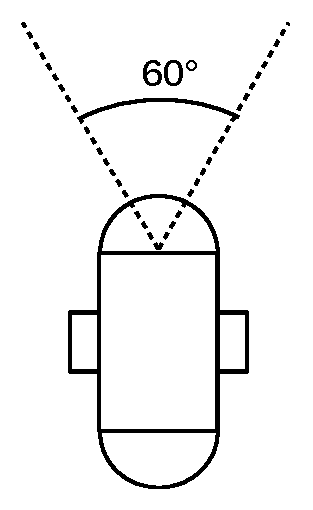
\includegraphics[height=0.7\textheight]{img/sensors_a.pdf}
					\caption{Infrared vision sensor}
					\label{fig:sensor_a}
				\end{figure}
				\onslide<2>
				\begin{figure}
					\centering
					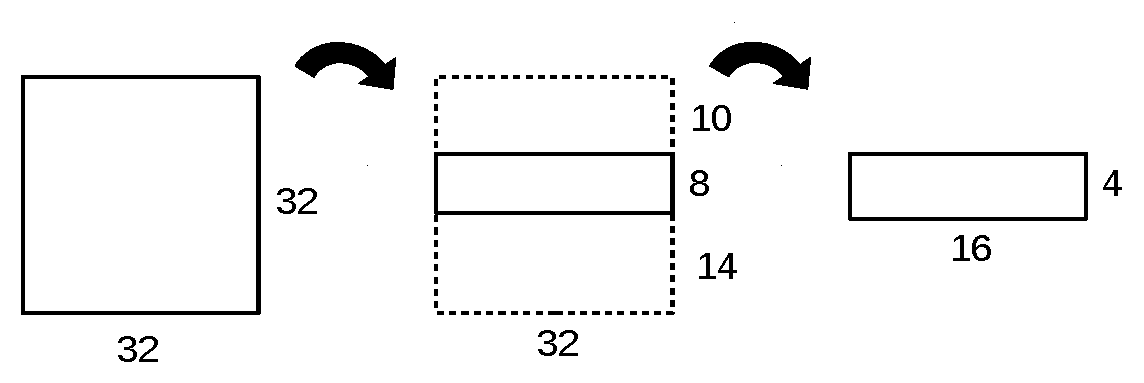
\includegraphics[width=\textwidth]{img/img_pre.pdf}
					\caption{Image preprocessing in 3 steps}
					\label{fig:img_pre}
				\end{figure}
				\onslide<3>
				\begin{figure}
					\centering
					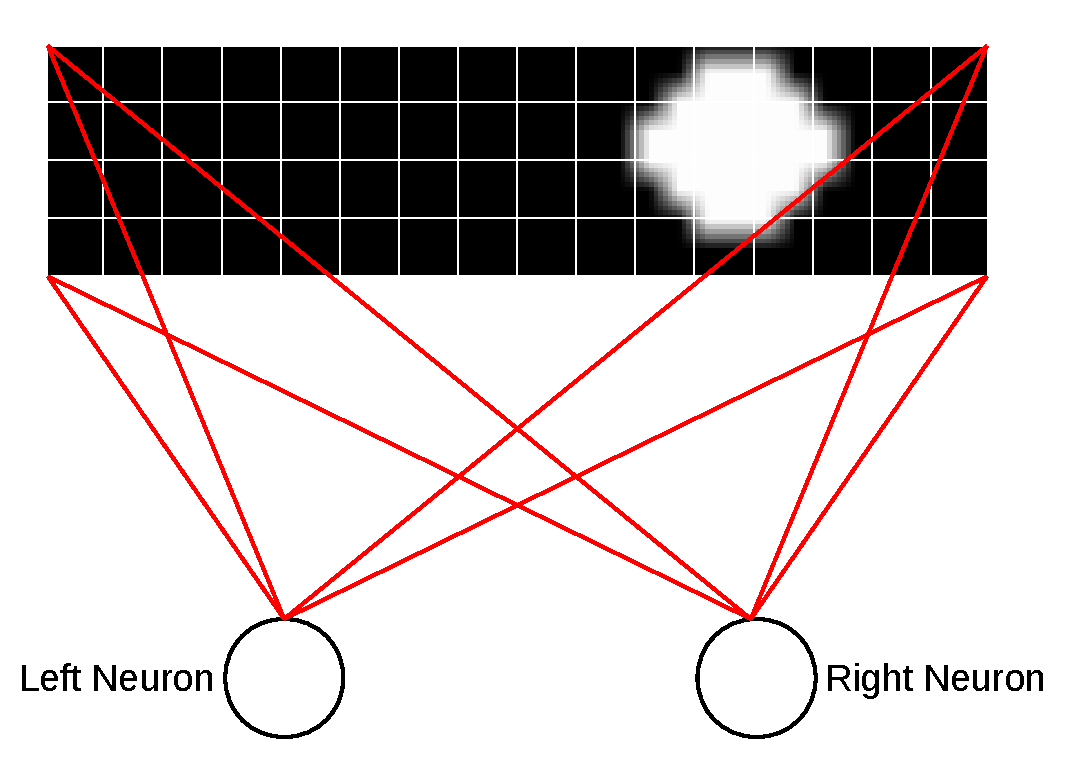
\includegraphics[width=\textwidth]{img/arch_tf.pdf}
					\caption{Target following SNN architecture}
					\label{fig:arch_tf}
				\end{figure}
			\end{overprint}
	\end{columns}
\end{frame}

\begin{frame}
	\frametitle{Target Following SNN cont.}
	\begin{columns}
		\column{0.5\linewidth}
			\begin{itemize}
				\item <1-> Output interpreted as angle
				\item <2-> Reward depends on Angle between head module and target
				\item <3-> Left and right neuron get the opposite rewards of each other
			\end{itemize}
		\column{0.5\linewidth}
			\begin{overprint}
				\onslide<1>
				\[decode\left(n_{spikes}\right) = \frac{n_{spikes}}{n_{max}}\]
				\[\alpha = \alpha_{max} \left(n_l - n_r\right)\]
				\[\alpha_t = c \alpha + \left(1 - c\right) \alpha_{t-1}\]
				\onslide<2>
				\begin{figure}
					\centering
					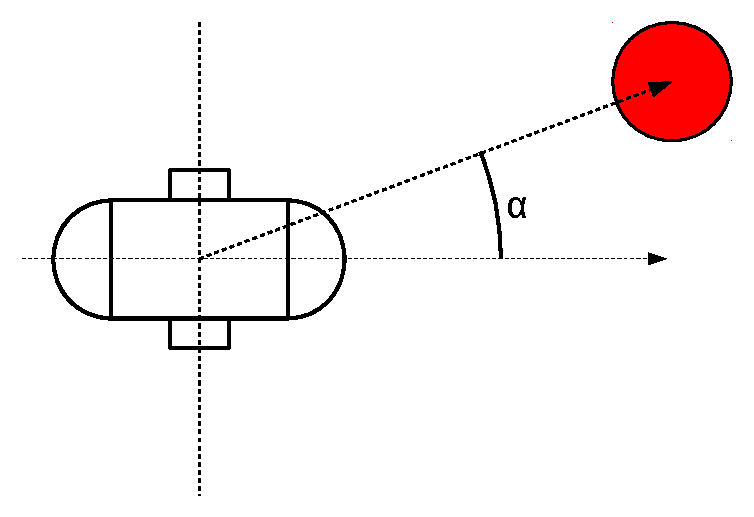
\includegraphics[width=\textwidth]{img/angle.pdf}
					\caption{Angle between robot head module and target.}
					\label{fig:angle}
				\end{figure}
				\onslide<3>
				\begin{figure}
					\centering
					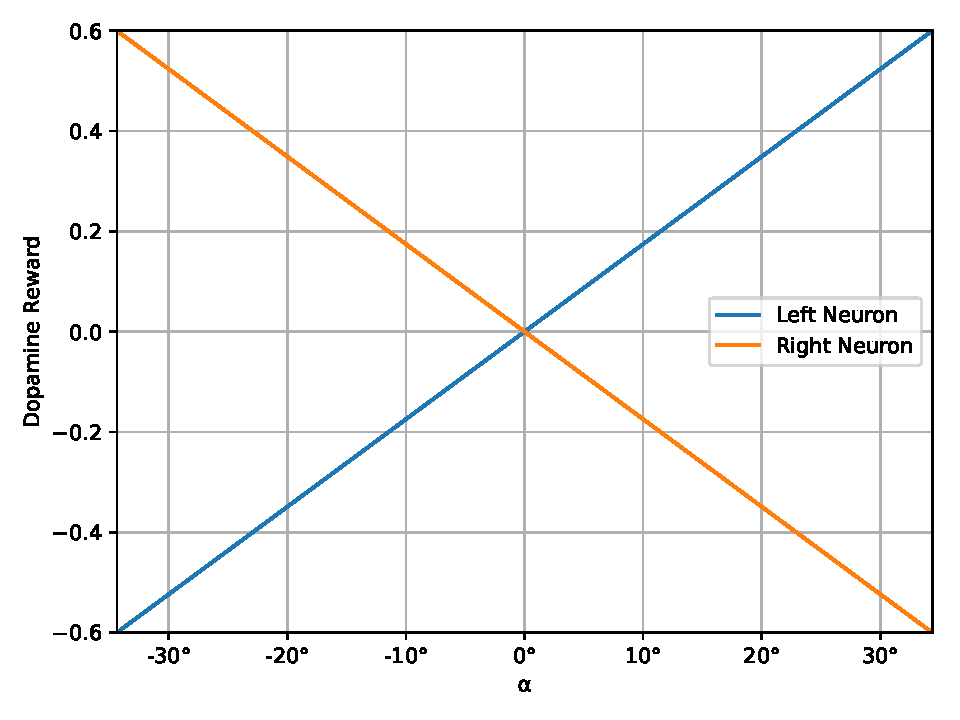
\includegraphics[width=\textwidth]{img/angle_reward.pdf}
					\caption{Target following reward function}
					\label{fig:angle_reward}
				\end{figure}
			\end{overprint}
	\end{columns}
\end{frame}

\begin{frame}
	\frametitle{Obstacle Avoidance SNN}
	\begin{columns}
		\column{0.5\linewidth}
			\begin{itemize}
				\item <1-> Four proximity sensors
				\item <2-> Proximity data preprocessing
				\item <3-> 4 Poisson input neurons
				\item <3-> Feed forward architecture
				\item <3-> Left and Right LIF output Neurons
			\end{itemize}
		\column{0.5\linewidth}
			\begin{overprint}
				\onslide<1>
				\begin{figure}
					\centering
					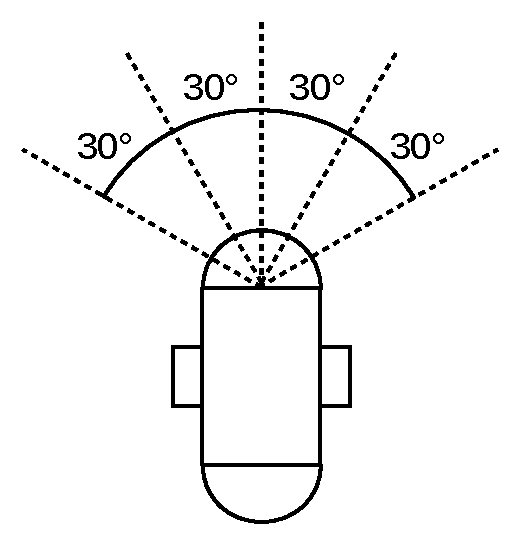
\includegraphics[height=0.7\textheight]{img/sensors_b.pdf}
					\caption{Proximity sensors}
					\label{fig:sensor_b}
				\end{figure}
				\onslide<2>
				\begin{itemize}
					\item Data in range $[0;3]$
					\item Mapped to range $[0:1]$
					\item $0$: No obstacle or at maximum distance
					\item $1$: Close obstacle
				\end{itemize}
				\onslide<3>
				\begin{figure}
					\centering
					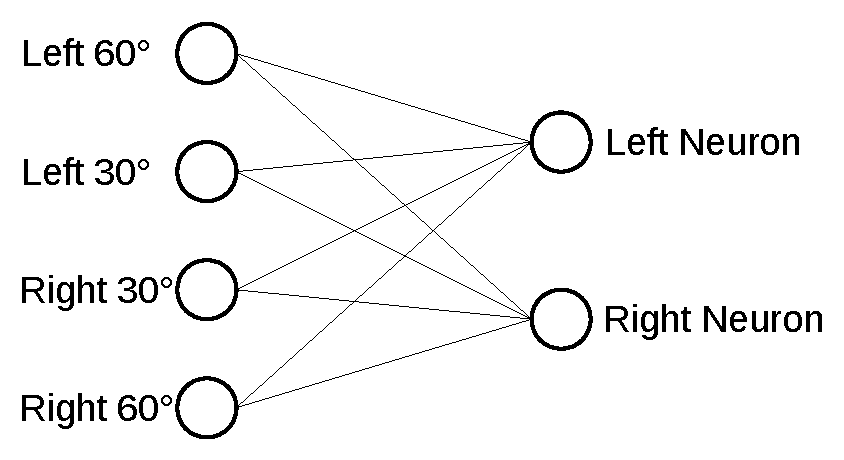
\includegraphics[width=\textwidth]{img/arch_oa.pdf}
					\caption{Obstacle avoidance SNN architecture}
					\label{fig:arch_oa}
				\end{figure}
			\end{overprint}
	\end{columns}
\end{frame}

\begin{frame}
	\frametitle{Obstacle Avoidance SNN cont.}
	\begin{columns}
		\column{\linewidth}
			\begin{itemize}
				\item <1-> Output interpreted as angle
				\[decode\left(n_{spikes}\right) = \frac{n_{spikes}}{n_{max}}\]
				\[\alpha = \alpha_{max} \left(n_l - n_r\right)\]
				\[\alpha_t = c \alpha + \left(1 - c\right) \alpha_{t-1}\]
				\item <2-> Event based rewards on Episode failure
				\item <2-> Left and right neuron get the opposite rewards of each other
				\item <2-> 4 Reward cases, collision and target lost, obstacle left or right side
			\end{itemize}			
	\end{columns}
\end{frame}

\begin{frame}
	\frametitle{Training}
	\begin{columns}
		\column{0.5\linewidth}
			\begin{itemize}
				\item <1-> Training environments
			\end{itemize}
		\column{0.5\linewidth}
			\begin{overprint}
				\onslide<1>
				\begin{figure}
					\centering
					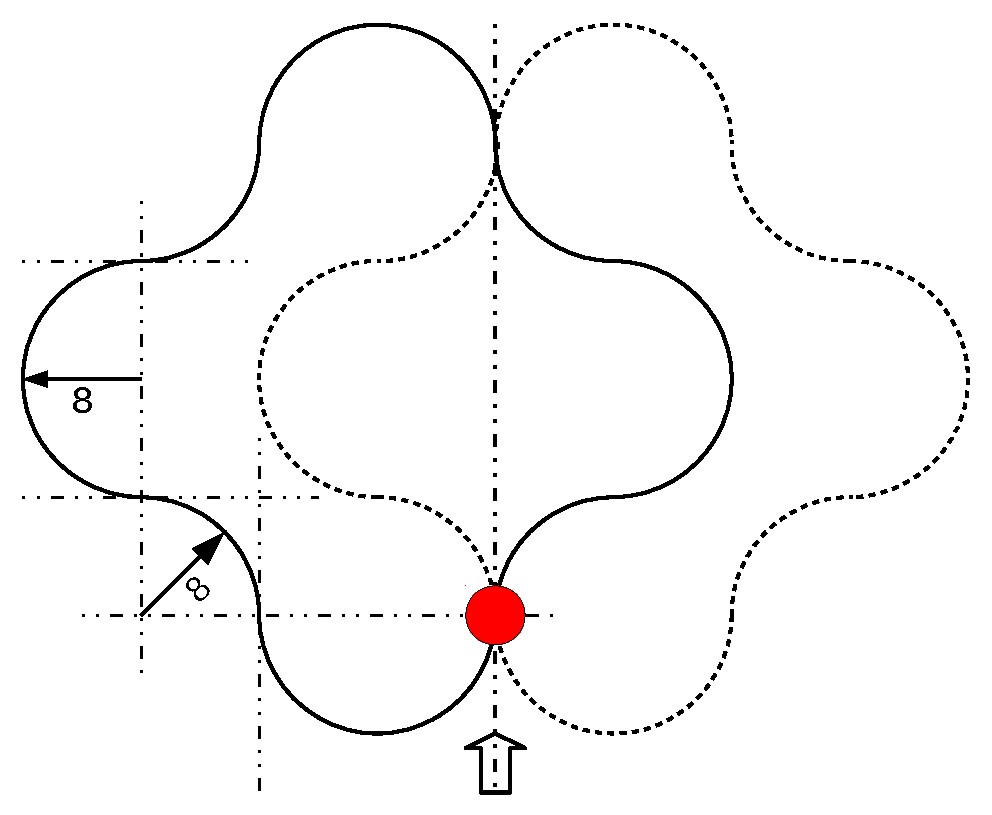
\includegraphics[width=\textwidth]{img/tf_training_path.pdf}
					\caption{Target tracking SNN training path.}
					\label{fig:tf_training_path}
				\end{figure}
				\onslide<2>
				\begin{figure}
					\centering
					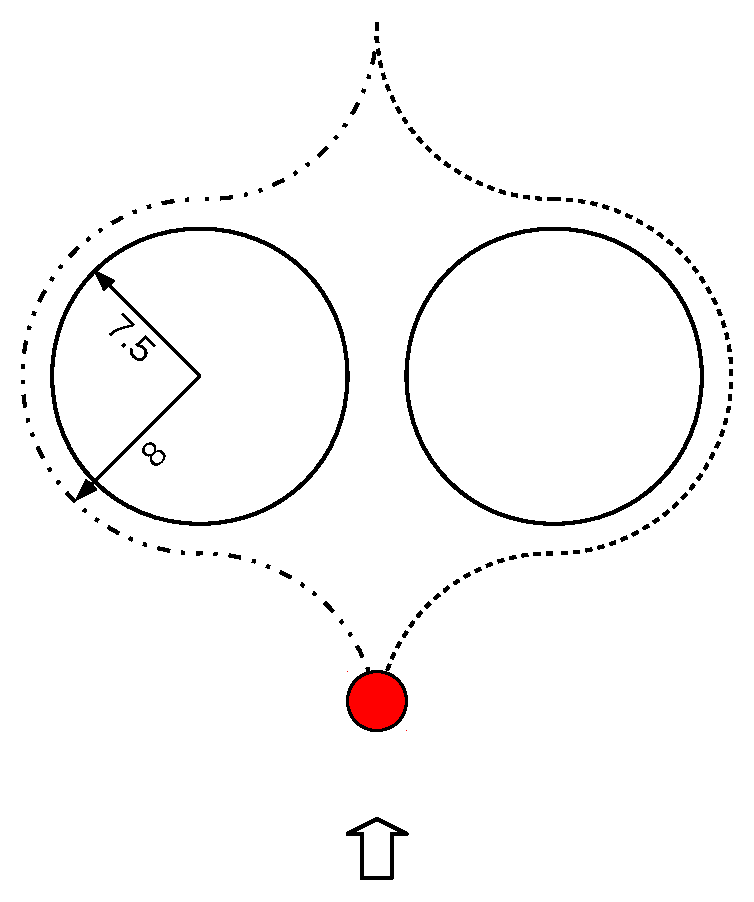
\includegraphics[height=0.6\textheight]{img/oa_training_path.pdf}
					\caption{Obstacle avoidance SNN training path.}
					\label{fig:oa_training_path}
				\end{figure}
			\end{overprint}
	\end{columns}
\end{frame}
